\section{Geneset Expansion}\label{sec:geneset_expansion}
As we said in \autoref{sec:introduction}, the only known responsible of the ZTTK disease, up to know, is the SON gene, even though it is a well known gene that contributes to the RNA splicing and the overall cell cycle. In order to study possible concurrent factor to the syndrome we have first enlarged the geneset under our focus (which we retrieved into a csv format from BioGRID \cite{biogrid} and cleaned by hand) by looking at all of the genes that interact with SON and, iteratively, also the second order neighbourhood. The request for the $1^{st}$ order neighbourhood retrieved 146 proteins and their (eventual) mutual interactions as we can see in \autoref{fig:starting_interactions} \subref{subfig:first_order_interactions}, the second request enlarged our network to $12863$ nodes.
\begin{figure}[H]
    \centering
    \subfloat[The $146$ starting interactions \label{subfig:son_interactions}]{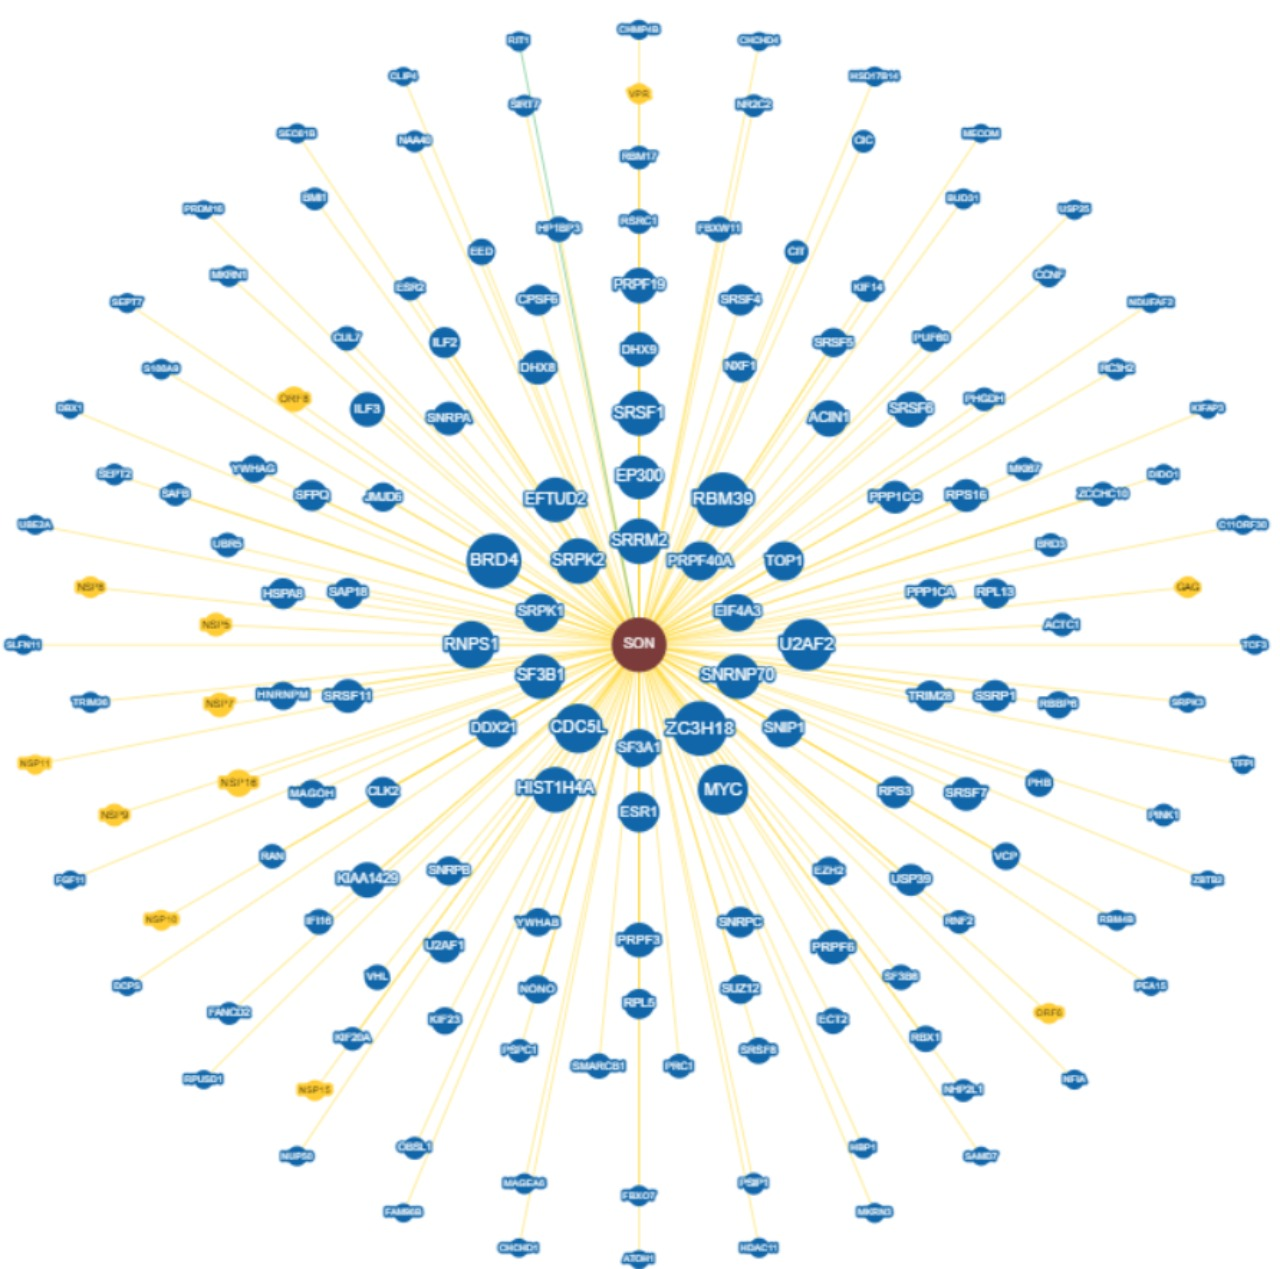
\includegraphics[width=0.5\linewidth]{images/geneset_starting_interactions.jpg}}
    \subfloat[The interactions at the first order \label{subfig:first_order_interactions}]{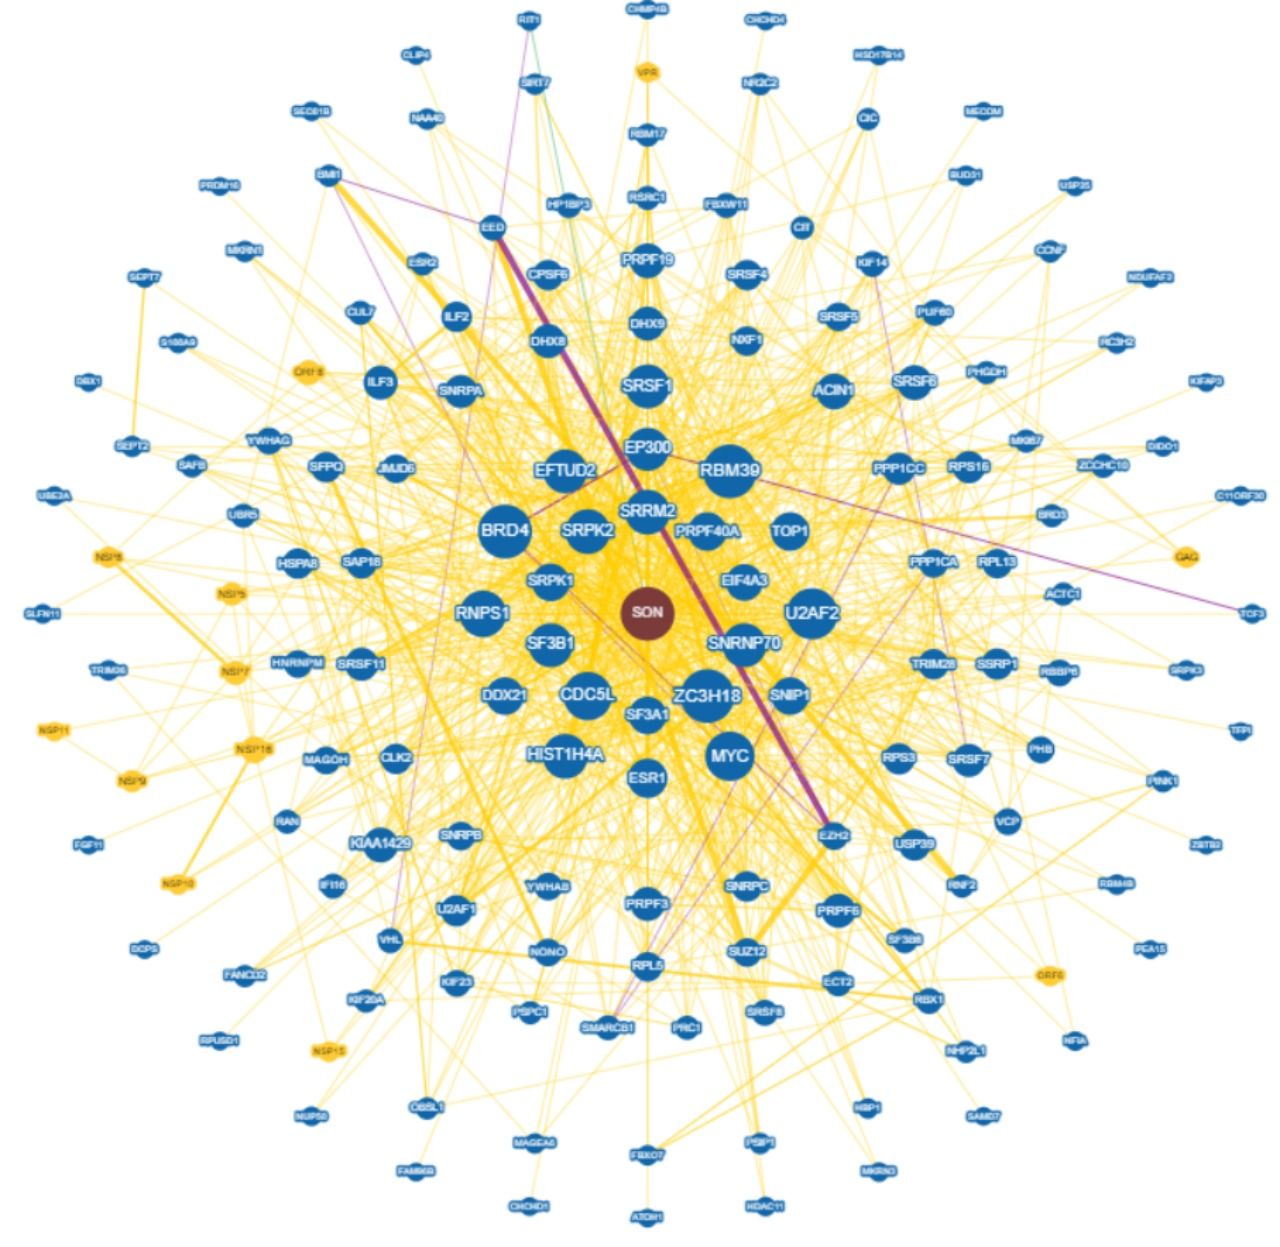
\includegraphics[width=0.5\linewidth]{images/geneset_first_order.jpg}}
    \caption{Starting interactions from the SON gene and all the first order interactions.}
    \label{fig:starting_interactions}
\end{figure}
All the information retrieved has been post-processed:
\begin{itemize}
    \item All the genes have been upper cased, the BioGRID dataset is mantained by its users, so we needed to uniform them;
    \item All the duplicated interactions were removed, there were $25281$ of such interactions and we did not them since our graph is not directed;
    \item All the self loops were removed, we are not interested in a protein interaction with itself.
\end{itemize}
As we can see in \autoref{fig:starting_interactions}, the shape of the network is well-defined, SON is at the center of the interactions and all of the nodes are distributed around it at a distance path of $2$, while two generic proteins can have a maximum distance of $4$. This graph is the starting point of our analysis, we have now a significant amount of data to perform a satisfying pathway enrichment 